\section{Edge Computing}
\label{sec:edge-computing}

The edge represents a new tier of infrastructure envisioned to address some of
the pitfalls with the cloud for IoT applications. Cisco named it ``the fog''
because the fog is a cloud close to the ground~\cite{bonomi2012fog}. CMU chose
``cloudlet'' to indicate this small-scale cloud datacenter~\cite{ha2014towards,
  satyanarayanan2009case}. At Berkeley, we use ``swarmbox'' to name the hardware
platform that accompanies swarm devices. Both Smartphones and Mini PCs mentioned
in~\autoref{sec:swarm-platforms} can act as edge computing platforms. We may
also expect compute infrastructure provided by carriers, such as central
offices\footnote{Often, a central office is defined as a building used to house
  the inside plant equipment of potentially several telephone exchanges, each
  serving a certain geographical area} or cell towers~\cite{att2017edge}.

As we illustrate in \autoref{fig:edge} The edge sits in the middle between
mobile/IoT devices and the cloud in terms of compute power. It needs to handle a
bit more workload, and incurs a slightly higher latency.

Researcher have begun exploring the benefit of edge platforms. For example, Kim
proposes an approach that leverages the edge computers as locally centralized
points for authentication and authorization to address IoT
security~\cite{kim2017securing}. Zhuo demonstrates how the edge infrastructure
can support computation offloading to achieve low
latency~\cite{chen2018application}. Mor et al.\,proposes a data-centric design
that focuses around the distribution, preservation, and protection of
information to address data privacy, scalability, durability,
etc~\cite{mor2016toward}.

\begin{figure}
  \centering
  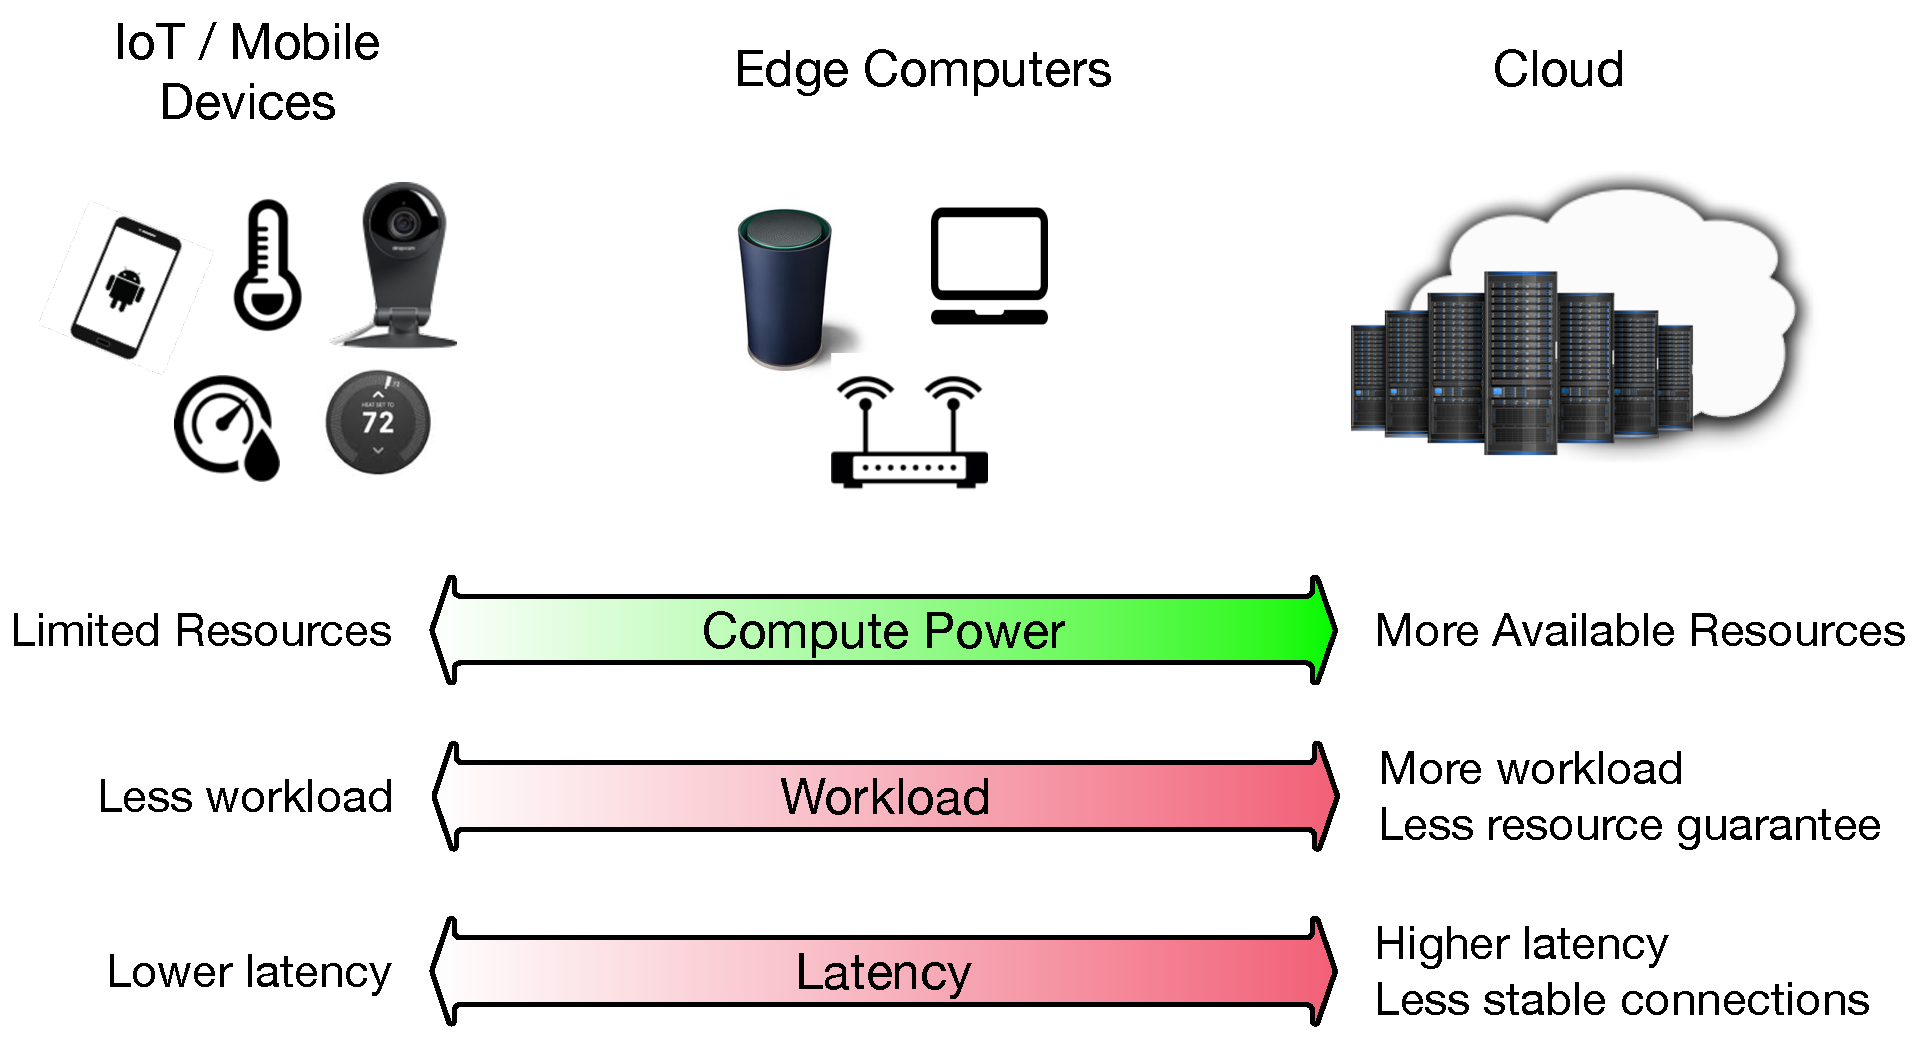
\includegraphics[width=0.85\textwidth]{figures/background.pdf}
  \caption{Mobile, Edge and the Cloud}
  \label{fig:edge}
\end{figure}

One form of the edge computers are gateways. Many gateways provide
application-specific connectivity for IoT devices to the Internet, bridging
low-power communication protocols such as BLE, 802.15.4 to IP. Even when devices
can utilize more standard communication protocols such as WiFi, the gateways
still exist as downloadable applications that run on cellphones or computers.

While an open gateway architecture can bring the benefit of the edge
computing~\cite{zachariah1001internet}., companies tend to provide their own
gateways, such as Ninja Sphere~\cite{ninja}, SmartThings Hub~\cite{smartthings},
Wink Hub~\cite{wink}. The fact that custom gateways are an integral part of
swarm applications leads directly to ``stovepipe'' solutions or
balkanization. Data and services from one company cannot be shared or utilized
by devices from another company: connection protocols, data formats, and
security mechanisms (when present) are proprietary and often undocumented.

% Researchers adopt a similar approach (e.g., HomeHub for the
% LoT~\cite{brush2013lab}).

%%% Local Variables:
%%% mode: latex
%%% TeX-master: "../background"
%%% End:
